\subsection{Ernst angle optimisation}
\label{subsec:poise__ernst}

\begin{figure}[htb]
    \centering
    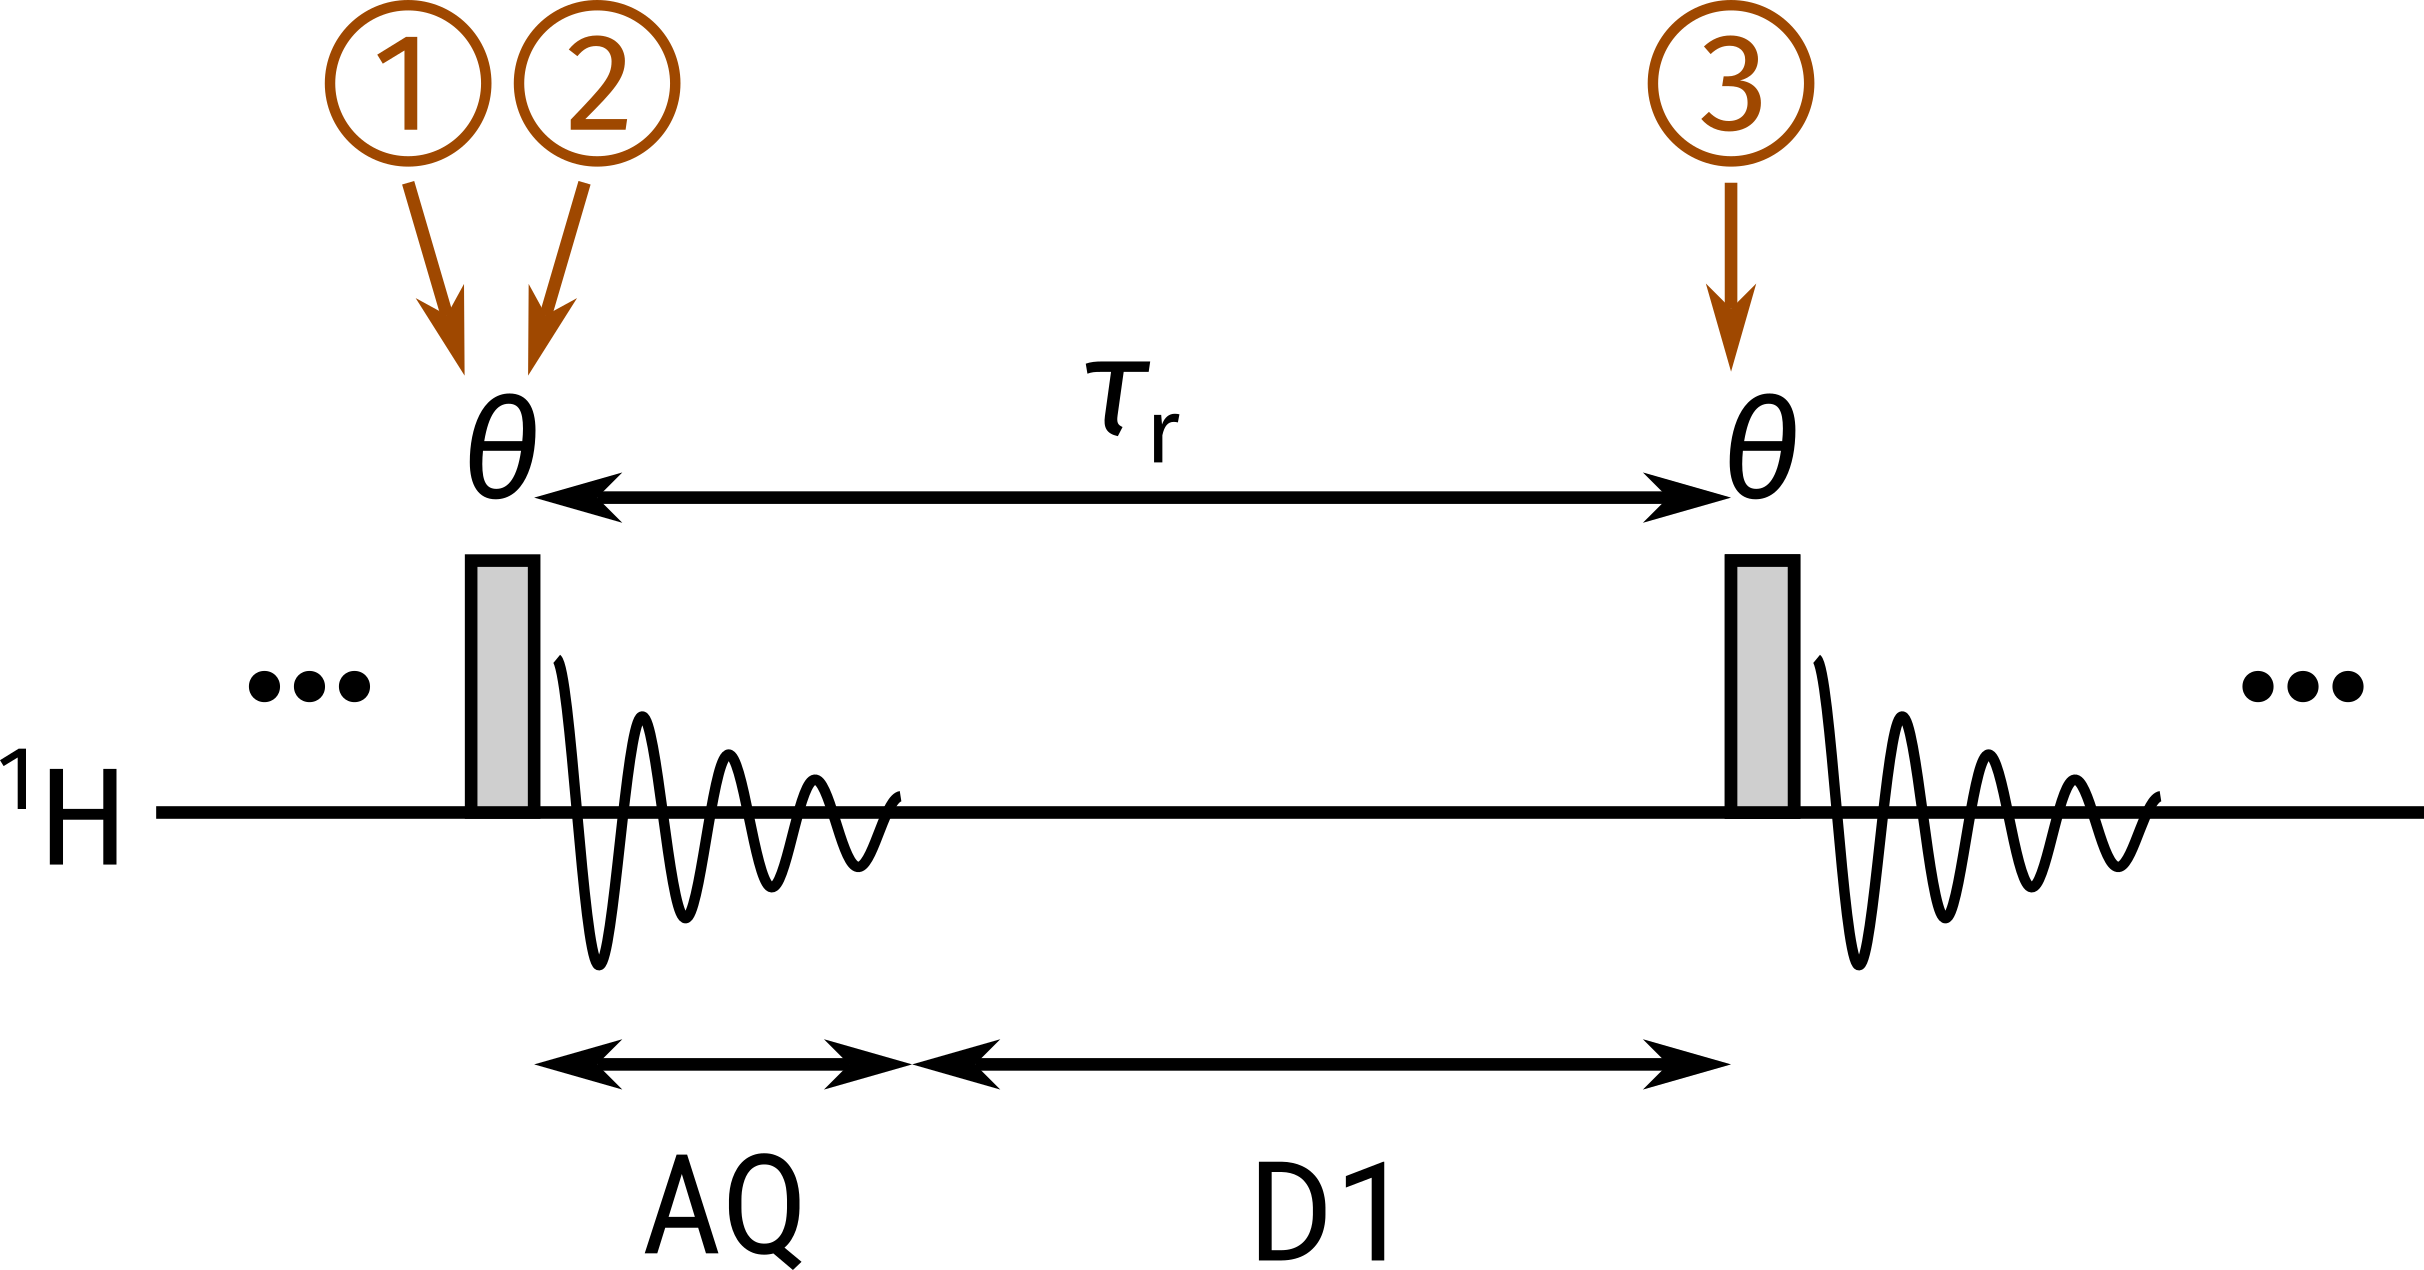
\includegraphics[]{pp/poise/zg_repeated.png}%
    \caption[Steady-state pulse--acquire experiment]{Steady-state pulse--acquire experiment. The excitation flip angle is $\theta$, and the repetition time between experiments is $\taur$.}
    \label{fig:zg_ernst}
\end{figure}

Often, in a simple 1D pulse--acquire spectrum it is not hugely important to know the exact \ang{90} pulse width: instead, it is more valuable to optimise the sensitivity per unit time of the spectrum.
Before launching straight into how this may be obtained through optimisation, it is instructive to first consider which parameters are worth optimising.
For a pulse--acquire experiment (\cref{fig:zg_ernst}), the repetition time $\taur$ is the sum of the acquisition time \texttt{AQ} plus the recovery delay \texttt{D1}; the flip angle $\theta$ is controlled via the pulse width \texttt{P1}.
We assume that the experiment has been repeated enough times to reach a \textit{steady state}, that is, the amount of $z$-magnetisation prior to the excitation pulse (point \circled{1}) is a constant, $M_{z,\text{ss}}$.
Application of the excitation pulse leads to a signal scaling as $M_{z,\text{ss}}\sin\theta$, and residual (unexcited) longitudinal magnetisation of $M_{z,\text{ss}}\cos\theta$ at point \circled{2}.
After the repetition time $\taur$ (point \circled{3}), it can be shown using the Bloch equations\autocite{Bloch1946PR} that the $z$-magnetisation recovers to
\begin{equation}
    \label{eq:z_magn_ernst1}
    M_{z,0}(1 - c) + cM_{z,\text{ss}}\cos\theta,
\end{equation}
where $c = \exp(-\taur/T_1)$ and $M_{z,0}$ is the initial, equilibrium $z$-magnetisation (before the experiment begins).
Since the experiment has reached a steady state, points \circled{1} and \circled{3} are equivalent: thus, we have that
\begin{equation}
    \label{eq:z_magn_ernst2}
    M_{z,0}(1 - c) + cM_{z,\text{ss}}\cos\theta = M_{z,\text{ss}},
\end{equation}
which can be rearranged to give
\begin{equation}
    \label{eq:z_magn_ernst3}
    \frac{M_{z,\text{ss}}}{M_{z,0}} = \frac{1 - c}{1 - c\cos\theta}.
\end{equation}
The signal amplitude $s$ therefore scales as
\begin{equation}
    \label{eq:z_magn_ernst4}
    s = \frac{(1 - c)}{1 - c\cos\theta} \cdot \sin\theta,
\end{equation}
and is maximised when $\md s/\md \theta = 0$, the solution of which is the celebrated \textit{Ernst angle}\autocite{Ernst1966RSI}:
\begin{equation}
    \label{eq:ernst_angle}
    \theta_\text{E} = \arccos{c} = \arccos\left[\exp\left(-\frac{\taur}{T_1}\right)\right].
\end{equation}
In general, $T_1$ and hence $\theta_\text{E}$ varies across the different spins in a given sample, so some degree of compromise is required in order to maximise sensitivity for all peaks.

To begin with, we may consider fixing $\taur$ and optimising \texttt{P1} to locate the Ernst angle (or to be precise, the pulse width which corresponds to the Ernst angle).
This is by no means an illogical proposition.
However, we can go one step further, because $\taur$ itself is comprised of two parameters, and the sensitivity \textit{per unit time} may be affected by varying $\taur$.
Since the signal scales as $1/\taur$ (a shorter $\taur$ means more repetitions per unit time) but the noise scales only as $\sqrt{1/\taur}$, the sensitivity per unit time is
\begin{equation}
    \label{eq:z_magn_ernst5}
    S = \frac{(1 - c)\sin\theta}{(1 - c\cos\theta)\sqrt{\taur}}.
\end{equation}
Assuming that $\theta$ is always set to the respective Ernst angle for different $\taur$, it can be shown that the best sensitivity per unit time is attained when $\taur \to 0$.\autocite{Waugh1970JMS,Traficante1992CMR}
Of course, this limit is not physically possible: $\taur$ comprises the acquisition time which must be nonzero.
However, it does imply that \texttt{AQ} should be kept as short as possible, and \texttt{D1} set to zero, as shown in \cref{fig:ernst_sensitivity}.

\begin{figure}[htb]
    \centering
    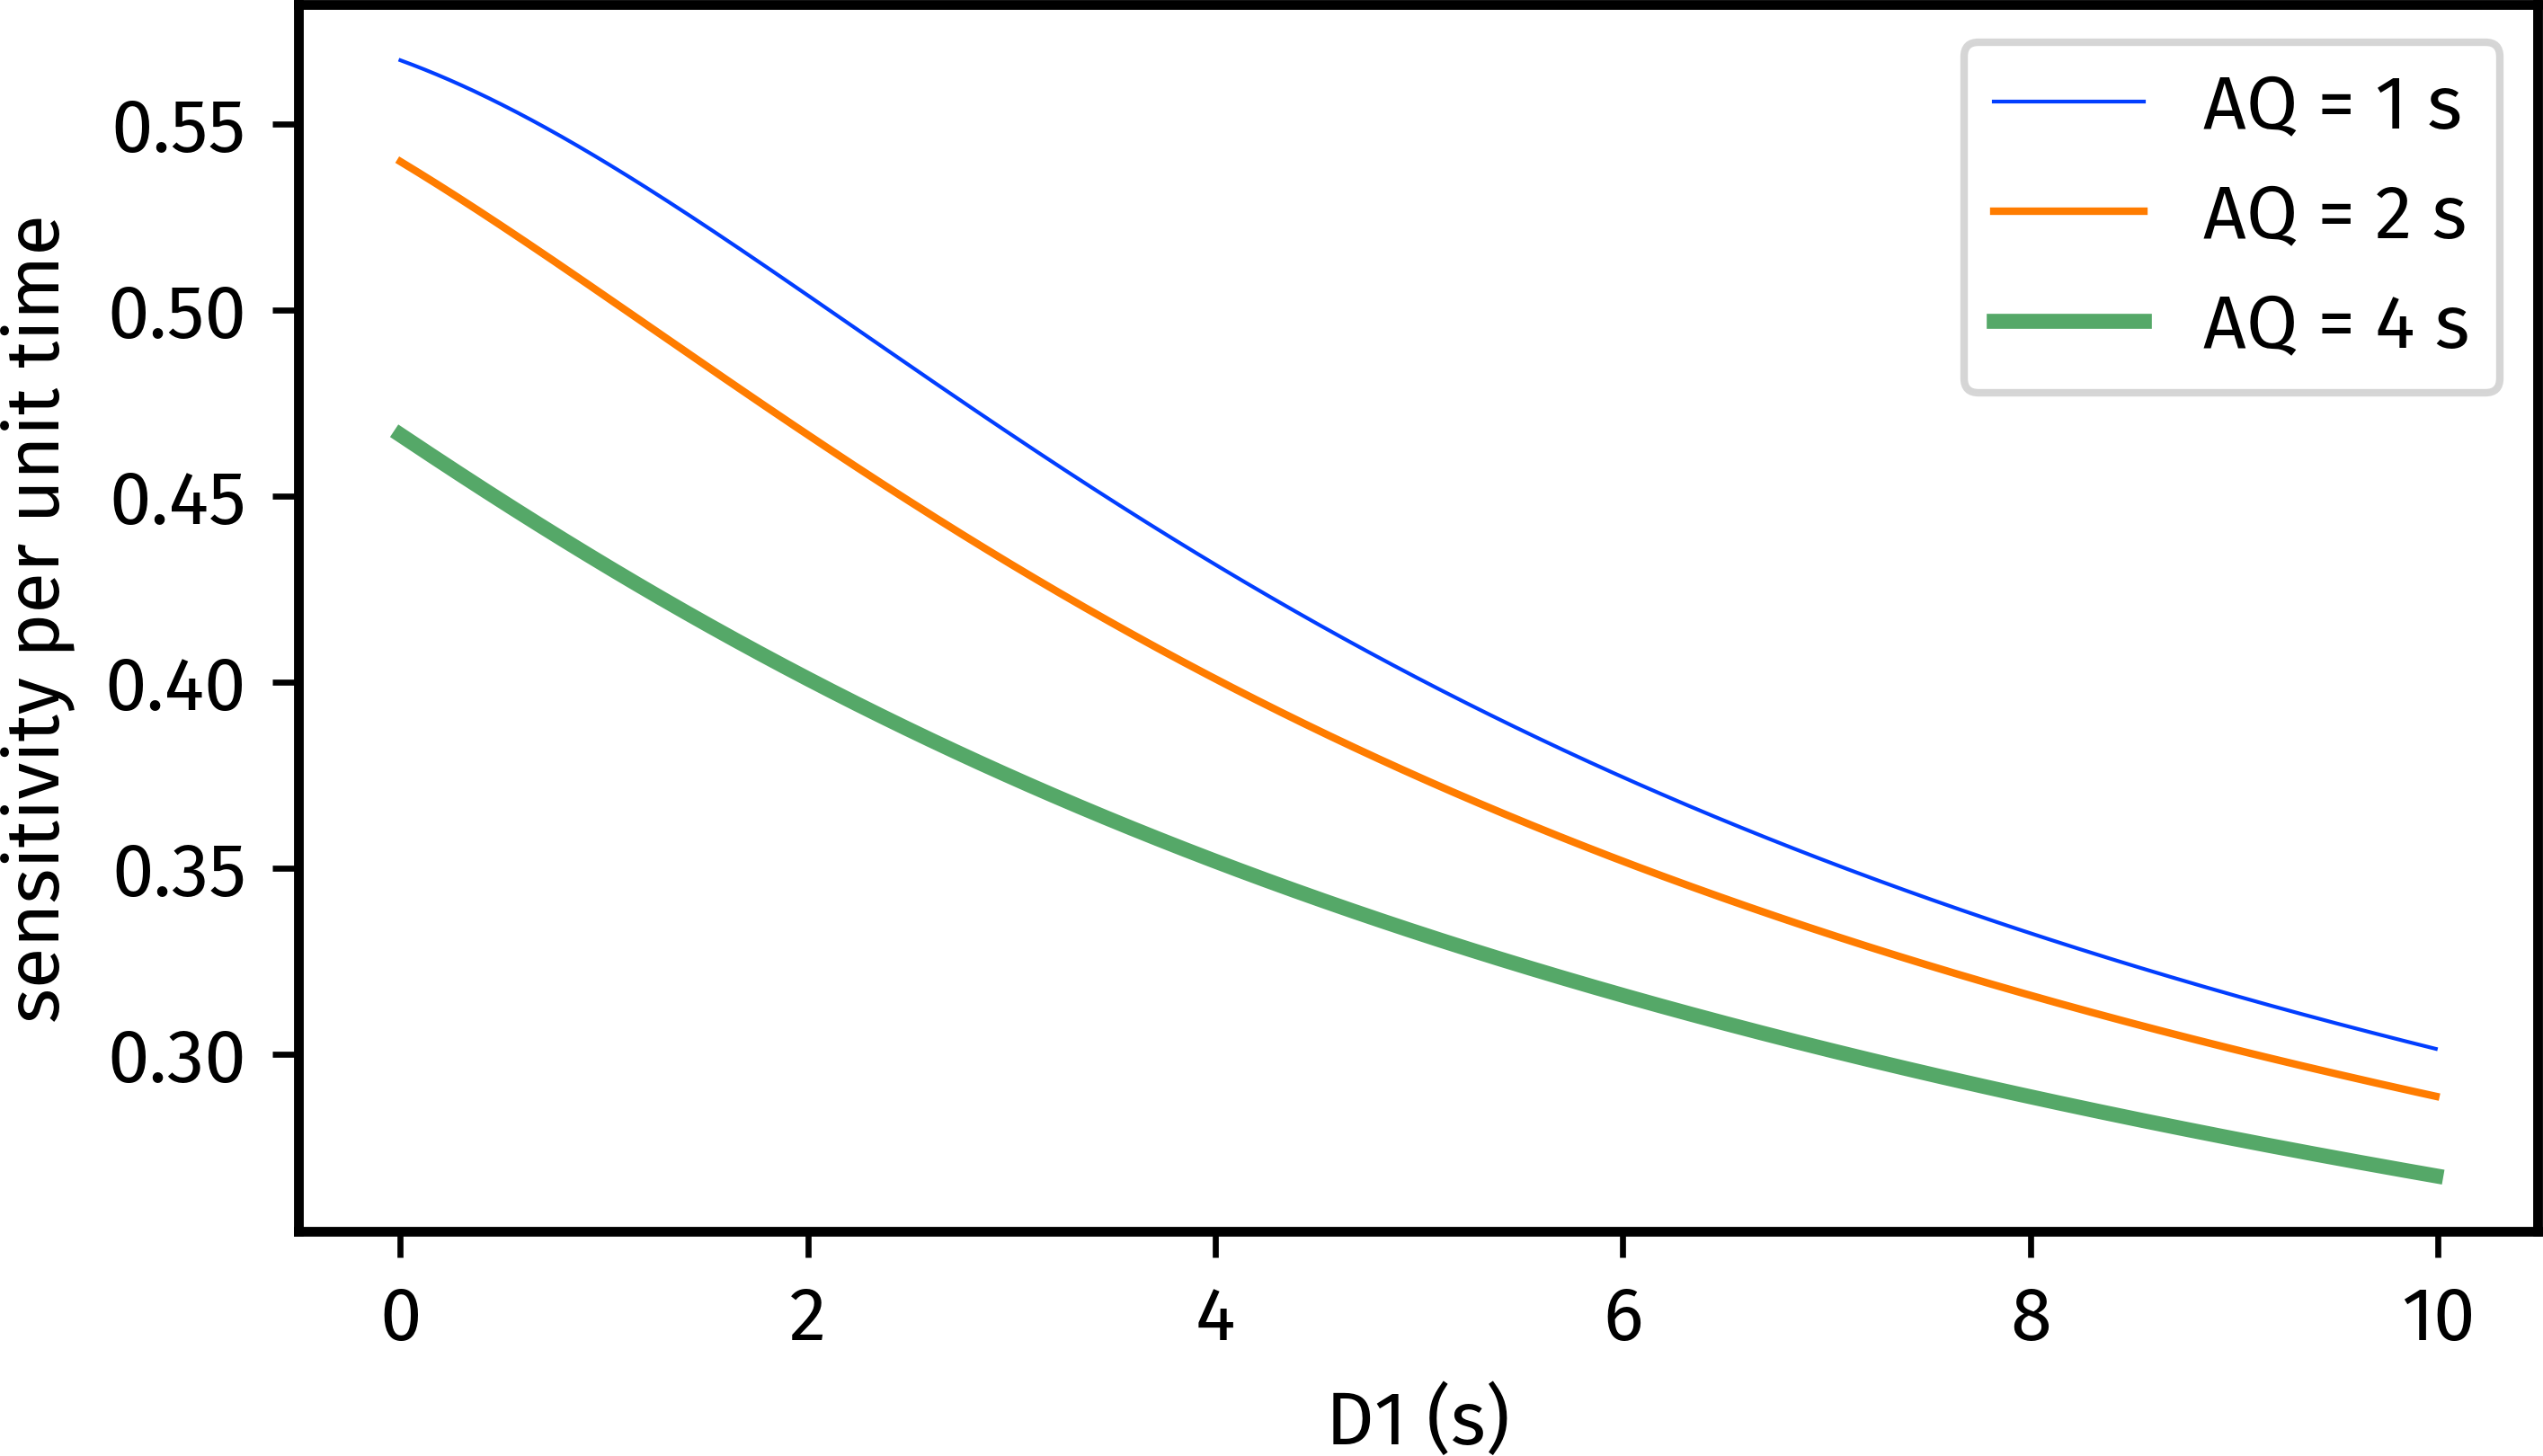
\includegraphics[]{poise/ernst_sensitivity.png}%
    \caption[Sensitivity per unit time as a function of \texttt{AQ} and \texttt{D1}]{Simulated sensitivity per unit time as a function of \texttt{AQ} and \texttt{D1} (as given by \cref{eq:z_magn_ernst5}), assuming that an Ernst angle excitation pulse is used. $T_1$ was set to \qty{1.5}{\s}.}
    \label{fig:ernst_sensitivity}
\end{figure}


\subsubsection{Optimisation setup}

Knowing this, we can then set up a meaningful optimisation routine.
We seek to optimise the pulse width \texttt{P1} such that the intensity of the real part of the spectrum is maximised (corresponding to a \texttt{maxrealint} cost function).
In practice, I took the extra step of calibrating the \ang{90} pulse width (as per the previous section) and modifying the pulse programme such that the flip angle could be specified as the parameter \texttt{CNST20}: this is not generally necessary and is only useful for evaluating the results, as will be shown later.
\texttt{AQ} and \texttt{D1} were set to be \qty{1.2}{\s} and 0 respectively, in accordance with the theory outlined above.
The number of scans (\texttt{NS}) can be set to 1, but unlike in the pulse width calibration (\cref{subsec:poise__pulsecal}), we must use enough dummy scans (\texttt{DS}) to ensure that a steady-state signal intensity is recorded: in practice I set \texttt{DS=4}.
This means that each FE, and thus the overall optimisation, requires a slightly longer time than the pulse width calibrations previously shown.


\subsubsection{Optimisation results}

The Ernst angle optimisation was run with two different spectral regions of interest: firstly, on all the aromatic and olefinic peaks in the sample of ferulic acid (\cref{tbl:poise_ernst_fivepeaks}), and secondly, on only a single peak at \qty{6.79}{\ppm} (\cref{tbl:poise_ernst_onepeak}).
(This spectral region can be selected using the TopSpin \texttt{dpl} command, which stores the bounds using the parameters \texttt{F1P} and \texttt{F2P}: all built-in cost functions respect these two parameters.)
Generally, optimisations could be completed in under two minutes.
The optima found for these two optimisations are different: this is because the former searches for a compromise Ernst angle which balances $T_1$ of all peaks within the region, and the latter optimises only for one $T_1$.

\begin{table}[htb]
    \hbadness=10000
    \centering
    \begin{tabular}{ccccc}
        \toprule
        Entry & Algorithm & Optimum found ($^\circ$) & FEs   & Time taken (\unit{\s}) \\
        \midrule
        1     & NM        & 67.5--73.1               & 9--13 & 91--132              \\
        2     & MDS       & 67.5--73.1               & 9     & 90--92               \\
        3     & BOBYQA    & 70.1--70.7               & 7     & 70--71               \\
        \bottomrule
    \end{tabular}
    \caption[Ernst angle optimisations on a range of peaks]{
        Ernst angle optimisation, performed on all aromatic and olefinic peaks in ferulic acid (between 6 and \qty{8}{\ppm}).
        The POISE routine used here is: \mintinline[breaklines]{json}{{"name": "ernst", "pars": ["cnst20"], "lb": [10.0], "ub": [90.0], "init": [30.0], "tol": [3.0], "cf": "maxrealint", "au": "poise_1d"}}.
        The mean of all five theoretical Ernst angles is \ang{65.2}.
        \datacode{5F-210619}
    }
    \label{tbl:poise_ernst_fivepeaks}
\end{table}

\begin{table}[htb]
    \hbadness=10000
    \centering
    \begin{tabular}{ccccc}
        \toprule
        Entry & Algorithm & Optimum found ($^\circ$) & FEs   & Time taken (\unit{\s}) \\
        \midrule
        1     & NM        & 60.0--67.5               & 9--11 & 91--111              \\
        2     & MDS       & 65.6--67.5               & 11    & 110--111             \\
        3     & BOBYQA    & 60.0--65.2               & 6--7  & 59--71               \\
        \bottomrule
    \end{tabular}
    \caption[Ernst angle optimisations on only one peak]{
        Ernst angle optimisations on the peak at \qty{6.79}{\ppm} in ferulic acid.
        The POISE routine is the same as in \cref{tbl:poise_ernst_fivepeaks}, but the spectral region under optimisation was set to be 6.71--\qty{6.87}{\ppm}.
        The theoretical optimum, as given in \cref{tbl:ernst_invrec}, is \ang{61.6}.
        \datacode{5F-210619}
    }
    \label{tbl:poise_ernst_onepeak}
\end{table}

To determine the accuracy of the optima found, rather than performing a reference grid search as in \cref{subsec:poise__pulsecal}, I measured $T_1$ of each of these peaks using a typical gradient-enhanced inversion--recovery experiment.
From this, the theoretical Ernst angles for each peak could be calculated (\cref{tbl:ernst_invrec}): they range from \ang{60} to \ang{73}.
The first optimisation, which should yield a weighted average of the five Ernst angles, appears at first glance to be biased towards the upper end of this range.
However, this can be rationalised by the fact that that a flip angle larger than $\theta_\text{E}$ is less detrimental to sensitivity compared to one that is smaller (this can be seen by plotting \cref{eq:z_magn_ernst4}).
On the other hand, the second optimisation yields an accurate value for the relevant peak (\ang{61.6}, peak number 4 in \cref{tbl:ernst_invrec}).

\begin{table}[!ht]
    \centering
    \begin{tabular}{ccccc}
        \toprule
        Peak & \proton{} chemical shift (ppm) & $T_1$ (\unit{\s}) & $\theta_\text{E}$ ($^\circ$) & $T_1\ln 2$ (\unit{\s})\\
        \midrule
        1 & 7.49 & 1.750 & 59.8 & 1.213 \\
        2 & 7.27 & 0.977 & 73.0 & 0.677 \\
        3 & 7.08 & 1.279 & 67.0 & 0.887 \\
        4 & 6.79 & 1.615 & 61.6 & 1.119 \\
        5 & 6.36 & 1.415 & 64.6 & 0.981 \\
        \bottomrule
    \end{tabular}
    \caption[$T_1$ values for ferulic acid]{
        $T_1$ and corresponding Ernst angles for each peak in ferulic acid, calculated for a repetition time of \qty{1.20}{\s}.
        Peak assignments can be found in \cref{chpt:assignments} \todo{Figure label maybe?}.
        The values of $T_1 \ln 2$, measured via a full pseudo-2D inversion--recovery experiment, are also provided here in anticipation of the optimisations in \cref{subsec:poise__invrec}.
        \datacode{5F-210619}
    }
    \label{tbl:ernst_invrec}
\end{table}

It is worth considering, though, whether this optimisation is truly worth it.
\proton{} pulse--acquire spectra already have a very high intrinsic sensitivity, and in the two minutes taken to optimise the flip angle, one could easily just acquire (around) 64 more scans, at which point knowledge of the Ernst angle would cease to be useful.
It \textit{may} be more useful for nuclei which have lower sensitivity, such as \carbon{}: I did not evaluate this possibility.
However, it must be borne in mind that a low-sensitivity experiment will also require more scans per FE, which leads to a corresponding increase in the optimisation time.

In my estimation, a more useful application of this optimisation routine would be to use it to determine an average $T_1$ value for a group of peaks.
This could then be used to inform the choice of recovery delay for multidimensional experiments\autocite{Reynolds2002JNP,Burns2021MRC} or quantitative NMR experiments\autocite{Pauli2005JNP,Giraudeau2014MRC}.
It is, however, possible to more directly obtain $T_1$ values from an inversion--recovery experiment, which I describe next.
